\documentclass{beamer}

\usetheme{Warsaw}
\usefonttheme{professionalfonts}
%\logo{\includegraphics[height=1cm]{./images/logo.png}}
\beamertemplatenavigationsymbolsempty
\setbeamertemplate{caption}{\raggedright\insertcaption\par}
\usepackage[T1]{fontenc}
\usepackage[utf8]{inputenc}
\usepackage[spanish]{babel}
\usepackage{float}
\usepackage{framed}
\usepackage{geometry}
\usepackage{tikz}
\usepackage{amssymb}
\usepackage{changepage}
\usepackage{xcolor}
\usepackage{minted}
\usepackage{fancyvrb}
\usepackage{relsize}
\usepackage{wasysym}
\usepackage{textcomp}
\usepackage{hyperref}
\usepackage{verbatim}
\usepackage{graphicx}
\usepackage{subcaption}
\definecolor{LightGray}{gray}{0.9}

%\setbeamertemplate{footline}[frame number]

\begin{document}

\title[Presentación del curso]{Teoría de la Computación \\ 2-2025}
\author[Teoría de la Computación]{Consuelo Ramírez \\ Cristóbal Loyola}
% \date{28 de marzo de 2025}
\date{}
\frame{\titlepage}

\begin{frame}{Resultados de aprendizaje general}
  Resolver problemas en contextos variados aplicando conceptos de la Teoría de
  la computación por medio de la representación y reconocimiento de
  \textbf{lenguajes formales, modelos de lógica clásica/difusa, computabilidad y
    complejidad computacional}; desarrollando la capacidad de adaptación a las
  condiciones de cada problema y los recursos disponibles, resguardando el
  compromiso con la ética y el trabajo bien realizado.
\end{frame}


\begin{frame}{Resumen del curso}
  \begin{itemize}[<+->]
    \item Desarrollar herramientas matemáticas para entender algoritmos y
          procesos computacionales.
    \item Analizar lenguajes formales y gramáticas, lo que es fundamental para
          entender el funcionamiento de lenguajes de programación y
          compiladores.
    \item Explorar qué significa que un problema sea computable, a través de
          modelos como autómatas y máquinas de Turing. Entender las
          limitaciones de estos modelos.
    \item Analizar los recursos (tiempo y espacio) requeridos para computar y
          clasificar problemas basado en su complejidad computacional.
  \end{itemize}
\end{frame}


\begin{frame}{Unidades}
  \begin{enumerate}[<+->]
    \item Lógica $\rightarrow$ (6 clases + 3 ayudantías)
    \item Lenguajes Regulares (LR)  $\rightarrow$ (8 clases + 3 ayudantías)
    \item Lenguajes Independientes del Contexto (LIC) $\rightarrow$ (6 clases +
          1 ayudantía)
    \item Computabilidad y Complejidad $\rightarrow$ (8 clases + 3 ayudantías)
  \end{enumerate}

\begin{figure}
    \centering
    \begin{subfigure}{0.24\textwidth}
        \centering
        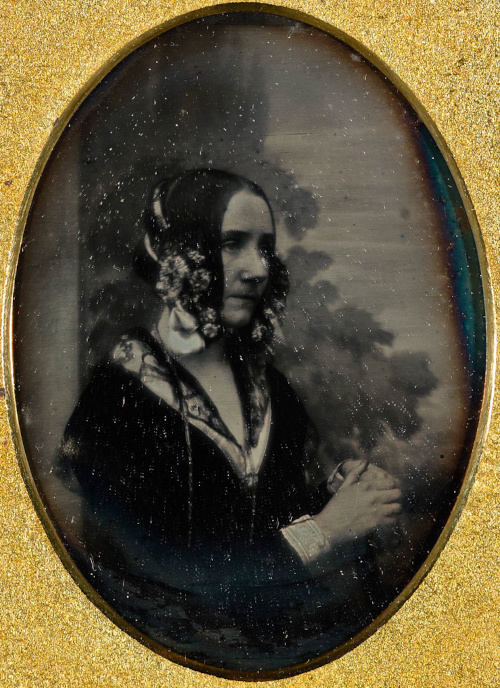
\includegraphics[width=\linewidth]{images/ada_lovelace.jpg}
    \end{subfigure}
    \hfill
    \begin{subfigure}{0.24\textwidth}
        \centering
        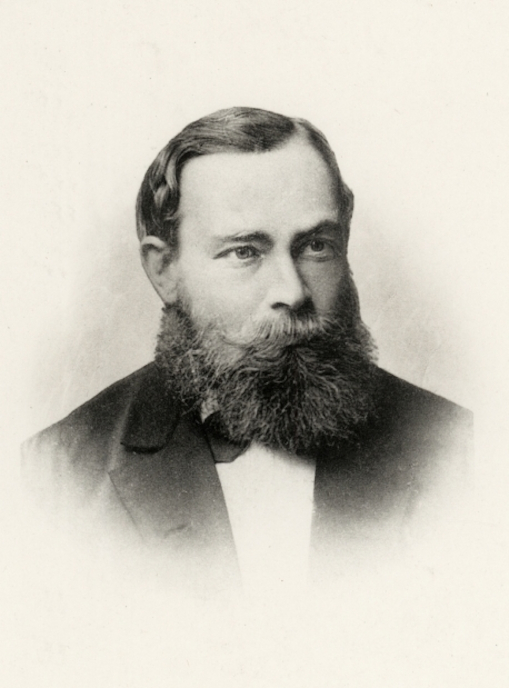
\includegraphics[width=\linewidth]{images/frege.jpg}
    \end{subfigure}
    \hfill
    \begin{subfigure}{0.24\textwidth}
        \centering
        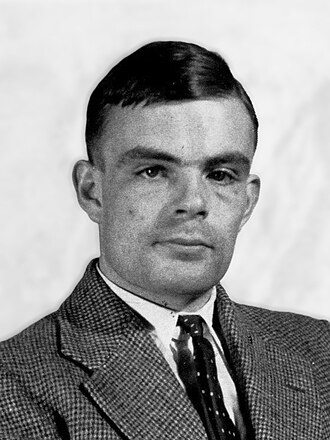
\includegraphics[width=\linewidth]{images/turing.jpg}
    \end{subfigure}
    \hfill
    \begin{subfigure}{0.24\textwidth}
        \centering
        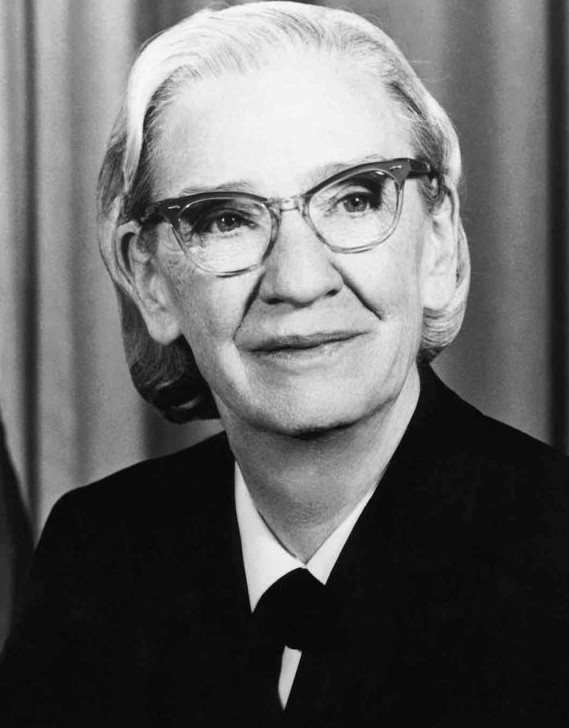
\includegraphics[width=\linewidth]{images/grace_hopper.jpg}
    \end{subfigure}
  \end{figure}
\end{frame}


\begin{frame}{Evaluaciones y asistencia}
  \begin{columns}
    \begin{column}{0.6\textwidth}
      \begin{itemize}
        \item \textbf{PEP 1} (15\%): 12 de septiembre
        \item \textbf{PEP 2} (30\%): 17 de octubre
        \item \textbf{PEP 3} (25\%): 7 de noviembre
        \item \textbf{PEP 4} (30\%): 2 de diciembre
      \end{itemize}
    \end{column}

    \begin{column}{0.4\textwidth}
      \begin{itemize}
        \item \textbf{PR}: 9 de diciembre
        \item \textbf{PDR}: 16 de diciembre
      \end{itemize}
    \end{column}
  \end{columns}

  \begin{itemize}[<+->]
    \vspace{0.3cm}
    \item El curso tiene 5 SCT y TEL: 4-2-0
    \item La condición para rendir la PDR es tener un promedio de PEPs mayor o
          igual que 3,0.
    \item La PDR reemplaza la calificación de la PEP que más desfavorece al
          promedio.
    \item La asistencia a clases es obligatoria en un 75\% como requisito de
          aprobación.
  \end{itemize}
\end{frame}


\begin{frame}{Bibliografía}
  \begin{itemize}
    \item Garrido, M. (2001). Lógica simbólica (4a ed.). Tecnos.
    \item Hopcroft, J., Motwani, R. y Ullman, J. (2002). Introducción a la
          Teoría de Autómatas, Lenguajes y Computación (2a ed.). Addison Wesley.
    \item Zhang, H., Zhang, J. (2024). Logic in Computer Science (2024th ed.).
          Springer.
    \item Sipser, M. (2013). Introduction to the Theory of Computation (3a ed.).
          Cengage Learning.
  \end{itemize}
\end{frame}

\end{document}
